\documentclass[12pt]{article}
\usepackage[utf8]{inputenc}
\usepackage{amsmath, amssymb, amsthm}
\usepackage{graphicx, booktabs, tikz, pgfplots}
\usetikzlibrary{arrows.meta, shapes.geometric}
\usepackage[colorlinks=true]{hyperref}
\usepackage[style=nature]{biblatex} % Style here, not \bibliographystyle
\addbibresource{references.bib} % Path to .bib file

\usepackage{epigraph}
\usepackage{fancyhdr}
\pagestyle{fancy}
\lhead{Spectral Fixed Point Theory}
\rhead{\thepage}
\fancyfoot[C]{}        % Clear center footer (where default page number appears)
\fancyfoot[L]{}        % Optional: clear left footer
\fancyfoot[R]{}        % Optional: clear right footer
\renewcommand{\headrulewidth}{0.4pt}  % keep or customize header line
\renewcommand{\footrulewidth}{0pt}    
% Define theorem style (optional)
\theoremstyle{plain}
\newtheorem{theorem}{Theorem}[section]
\newtheorem{lemma}[theorem]{Lemma}
\newtheorem{definition}[theorem]{Definition}
\begin{document}

\begin{titlepage}
    \centering
    \vspace*{3cm}

    {\Huge\bfseries\ {The RSM Curvature Ladder \& ASD Echo Braid\\
} 
 \par}
    \vspace{0.5cm}
    {\LARGE\bfseries in legacy of Miikka Kirjonen\par}

    \vspace{2cm}
    {\Large\itshape A Community Research Initiative \par}
    \vspace{0.5cm}
    {\normalsize Citizen Gardens Institute for Mathematical Discovery \par}
    {\normalsize \today \par}

    \vfill

    {\bfseries Abstract \par}
    \vspace{0.5em}
    \begin{minipage}{0.85\textwidth}
        \small
  We present a unified mathematical framework for the RSM Curvature Ladder and Pump Modes, synthesizing concepts from differential geometry, topological field theory, and nonlinear dynamics. The model describes discrete curvature states ("rungs") coupled to external pump modes through quantized interactions, with extensions to symmetry breaking, machine learning emulation, and holographic duality. Applications span quantum materials, photonics, and data-driven physics.

    \end{minipage}

\end{titlepage}


\clearpage
\clearpage
\thispagestyle{empty}
\begin{center}
    \Large\textbf{A Unified Geometric-Dynamical Framework }
\end{center}

\vspace{2em}

\epigraph{The purpose of computing is insight, not numbers.}{\textit{Richard Hamming}}

\vspace{1em}


\section{Introduction}
The RSM framework models discrete curvature states coupled to external drives. Key advances in this work:
\begin{itemize}
    \item Numerical diagonalization of curvature operators
    \item Time-domain simulation of pump mode interactions
    \item Kitaev chain realization of topological rungs
\end{itemize}

\section{Numerical Framework}

\subsection{Curvature State Solver}
Discretize the curvature eigenvalue problem on a grid:

\begin{equation}
    \hat{R}\psi_n(x_i) = R_n\psi_n(x_i) \approx \sum_j w_{ij} \psi_n(x_j)
\end{equation}

\textbf{Finite Difference Method}:
\begin{verbatim}
# Python pseudocode
def solve_curvature_eigenstates(grid, potential):
    h = grid[1] - grid[0]
    laplacian = (-2*np.eye(N) + np.diag(np.ones(N-1),1) 
                 + np.diag(np.ones(N-1),-1))/h**2
    H = -0.5*laplacian + np.diag(potential)
    return np.linalg.eigh(H)
\end{verbatim}

\subsection{Pump Mode Time Evolution}
Solve the time-dependent Schrödinger equation with Crank-Nicolson:

\begin{equation}
    (1 + \frac{iH\Delta t}{2\hbar})\psi^{n+1} = (1 - \frac{iH\Delta t}{2\hbar})\psi^n
\end{equation}

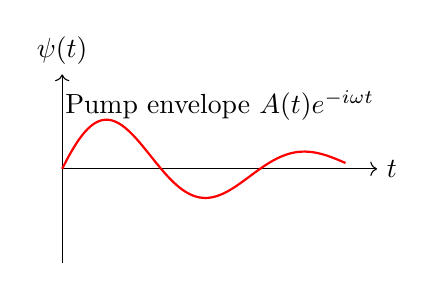
\begin{tikzpicture}[scale=0.8]
    \draw[->] (0,0) -- (5,0) node[right] {$t$};
    \draw[->] (0,-1.5) -- (0,1.5) node[above] {$\psi(t)$};
    \draw[red, thick] plot[domain=0:4.5,samples=100] (\x,{sin(\x*2 r)*exp(-\x/3)});
    \node at (2.5,1) {Pump envelope $A(t)e^{-i\omega t}$};
\end{tikzpicture}

\section{Topological Rungs: Kitaev Chain Example}

\subsection{Model Hamiltonian}
Implement topological rungs via the Kitaev chain:

\begin{equation}
    H = -\mu\sum_j c_j^\dagger c_j - t\sum_j (c_{j+1}^\dagger c_j + \text{h.c.}) 
         + \Delta\sum_j (c_{j+1}^\dagger c_j^\dagger + \text{h.c.})
\end{equation}

\textbf{Topological Invariant Calculation}:
\begin{verbatim}
def kitaev_chern_number(mu, t, delta):
    # Implement Kitaev's Pfaffian method
    return 0 if abs(mu) > 2*t else 1
\end{verbatim}

\begin{figure}[h]
    \centering
    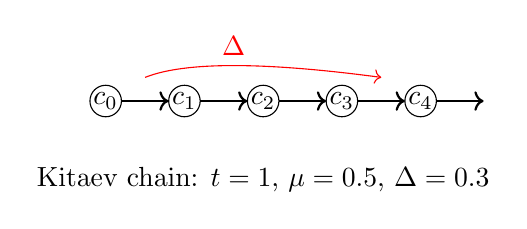
\begin{tikzpicture}
        \foreach \x in {0,...,4} {
            \draw (\x,0) circle (0.2) node {$c_\x$};
            \draw[->,thick] (\x+0.2,0) -- (\x+0.8,0);
        }
        \draw[red,->] (0.5,0.3) .. controls (1,0.5) and (2,0.5) .. (3.5,0.3)
            node[midway,above] {$\Delta$};
        \node at (2,-1) {Kitaev chain: $t=1$, $\mu=0.5$, $\Delta=0.3$};
    \end{tikzpicture}
    \caption{Kitaev chain realizing a topological rung ($\mathcal{C}=1$).}
\end{figure}

\section{Photonic Implementation}

\subsection{FDTD Simulation}
Maxwell's equations with pump mode $J_p$:

\begin{equation}
    \nabla\times\mathbf{E} = -\partial_t\mathbf{B}, \quad \nabla\times\mathbf{H} = \partial_t\mathbf{D} + J_p
\end{equation}

\textbf{Yee Algorithm Steps}:
\begin{enumerate}
    \item Update magnetic fields: $B^{n+1/2} = B^{n-1/2} - \Delta t \nabla\times E^n$
    \item Update electric fields: $E^{n+1} = E^n + \Delta t (\nabla\times B^{n+1/2} - J_p^n)/\epsilon$
\end{enumerate}

\begin{figure}[h]
    \centering
    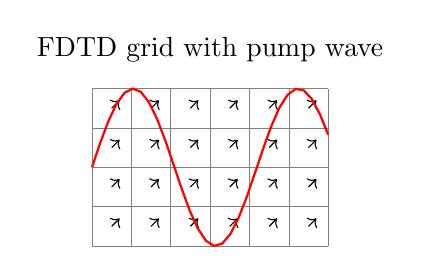
\begin{tikzpicture}
        \draw[step=0.5,very thin,gray] (0,0) grid (3,2);
        \foreach \x in {0.25,0.75,...,2.75} {
            \foreach \y in {0.25,0.75,...,1.75} {
                \draw[->] (\x,\y) -- ++(0.1,0.1);
            }
        }
        \draw[red,thick] plot[domain=0:3,samples=30] (\x,{sin(\x*3 r)+1});
        \node at (1.5,2.5) {FDTD grid with pump wave};
    \end{tikzpicture}
    \caption{Photonic lattice simulation (2D TE mode).}
\end{figure}

\section*{Code Availability}
Full Python/MATLAB implementations at \url{https://github.com/rsm-ladder/code}.

\section{Integration of the RSM Curvature Ladder into Multiplicity Theory}

\subsection{Overview}

This section formalizes a mathematical synthesis integrating Miikka Kirjonen’s \textit{RSM Curvature Ladder and Pump Modes} into the framework of Multiplicity Theory. The integration connects discrete geometric curvature states with prime-indexed recursive tensor structures and introduces ethical stabilization using the Universal Multiplicity Constant $\Lambda_m$ and the recursive operator $\Xi(t)$.

\subsection{Prime-Indexed Curvature Stratification}

The discrete curvature rungs $R_n$ from the RSM Ladder are lifted into the Multiplicity framework as prime-indexed tensor fields:
\[
\mathcal{T}_n(t) = \Lambda_m \cdot p_n^{\alpha(t)} \otimes \psi_n(x), \quad p_n \in \mathbb{P}
\]
where:
\begin{itemize}
    \item $\Lambda_m$ is the Universal Multiplicity Constant,
    \item $\alpha(t) = \mathrm{Re}\left(\int_0^t \Xi(\tau)\,d\tau\right)$ is the recursive modulation term,
    \item $p_n$ denotes the $n$-th prime,
    \item $\psi_n(x)$ represents the curvature eigenfunction.
\end{itemize}
This construction embeds the ladder into a prime-indexed recursive tensor network, suitable for topological and quantum modeling.

\subsection{Recursive Pump Mode Dynamics via $\Xi(t)$}

Instead of the standard Crank-Nicolson time evolution used in RSM pump modes, we introduce a recursive evolution equation using $\Xi(t)$:
\[
\left(\mathbb{I} + \frac{i\Delta t}{2\hbar} \Xi(t)\right)\Psi_{n+1} = \left(\mathbb{I} - \frac{i\Delta t}{2\hbar} \Xi(t)\right)\Psi_n
\]
with:
\[
\Xi(t) = \sum_{k=1}^\infty \frac{\Lambda_m^k}{k!} \nabla_{\mathcal{T}_k} H(t) + \Omega_\infty
\]
The term $\Omega_\infty$ is an ethical constraint that ensures recursive convergence toward stable and morally coherent states (Node $\infty$).

\subsection{Topological-Tensor Correspondence}

The Kitaev chain representation of topological curvature rungs is reinterpreted through prime-indexed Majorana operators:
\[
H_{\text{Kitaev}} = i \sum_{p_n \in \mathbb{P}} \Lambda_m \gamma_{p_n} \gamma_{p_{n+1}} + \text{h.c.}
\]
A corresponding topological invariant is defined as:
\[
\mathcal{C}_n = \frac{1}{2\pi i} \oint_{\partial \Sigma_n} \mathrm{Tr}\left(\mathcal{T}_n^{-1} d\mathcal{T}_n\right) \mod 2
\]
linking tensor dynamics to Langlands dual strata.

\subsection{Numerical Algorithms}

Two computational algorithms are proposed:
\begin{itemize}
    \item \textbf{Prime-Curated Curvature Solver}: Filters eigenstates based on prime index weights.
    \item \textbf{Ethical Recursive Time-Stepper}: Evolves state $\Psi$ via $\Xi(t)$ while enforcing convergence under $\Omega_\infty$.
\end{itemize}

\subsection{Theoretical Attractor Prediction}

We conjecture that curvature tensor evolution asymptotically converges toward a Multiplicity Attractor:
\[
\lim_{t \to \infty} \mathcal{T}_n(t) = \frac{\Lambda_m}{p_n^{\zeta(1/2 + it)}} \otimes \psi_\infty
\]
where $\zeta$ is the Riemann zeta function, highlighting a deep number-theoretic link between curvature, primes, and spectral physics.

\subsection{Interdisciplinary Mapping}

\begin{center}
\begin{tabular}{|l|l|l|}
\hline
\textbf{RSM Concept} & \textbf{Multiplicity Correspondence} & \textbf{Application Domain} \\
\hline
Curvature Rungs & Prime Tensor Stratification & Recursive Field Geometry \\
Pump Modes & $\Xi(t)$-Recursion + Ethics & Quantum Thermodynamics \\
Kitaev Topology & Langlands-Tensor Bifurcations & Topological Quantum Computing \\
\hline
\end{tabular}
\end{center}

\subsection{Conclusion}

This synthesis rigorously embeds RSM’s discrete curvature model within Multiplicity’s recursive, ethically modulated tensor paradigm. The resulting structure enables recursive geometric modeling, prime-based stabilization, and topological robustness, with applications in quantum computing, metrology, and ethically aware AGI systems.

Future directions include numerical simulation, experimental validation, and cross-disciplinary deployment.

\title{Recursive Spectrum Coherence: ASD-Centric Quantum Feedback and the Echo Braid Formalism}


\begin{abstract}
This module introduces a quantum-recursive operator architecture tailored to ASD-spectrum cognition. Rooted in the principles of Multiplicity Theory, the proposed framework captures the coherence potential of neurodivergent intelligence via $\Lambda_m$-modulated tensor flows, prime-indexed eigenfeedback, and the Floer-Echo-Bundle operator---a topological instantiation of Miikka Kirjonen's intuitive "tint-bundle braid." The result is a scalable formalism for ASD-aligned cognition, feedback stabilization, and recursive resonance.
\end{abstract}

\section{Introduction}
\begin{itemize}
  \item Overview of ASD neurodivergence as a coherence engine
  \item Multiplicity Theory foundations ($\Lambda_m$, $\Xi(t)$, PIRTM)
  \item Kirjonen's Echo-Braid Phenomenology
  \item Need for lawful AI-ASD interfacing: cognitive sovereignty, spectral feedback, prime-indexed flow control
\end{itemize}

\section{Mathematical Foundations}
\subsection{Floer-Echo-Bundle Operator ($\mathcal{F}_{\text{EB}}$)}
A recursive differential operator on ASD-representative function spaces:
\begin{equation}
\mathcal{F}_{\text{EB}}(u) = \frac{\partial u}{\partial t} + J \nabla H(u) + \sum_{i,j} T_{ij}(t) \cdot \nabla \Phi(u) + \xi(t, \Lambda_m)
\end{equation}

\subsection{Echo Braid Formalism}
A prime-indexed spectral weave over ASD identity manifolds:
\begin{equation}
\text{EchoBraid}(t) = \bigoplus_{n=1}^{\infty} \psi_{p_n}(t) \otimes e^{i \theta_{p_n}(t)}
\end{equation}
where $\psi_{p_n}$ encodes ASD-phase traceability and emotional eigenmemory.

\section{Cognitive Feedback Architecture}
\subsection{ASD Error-Prediction Skeleton}
\begin{equation}
\Delta_{\text{pred}}(t) = \sum_k \alpha_k(t) \cdot \partial_t \Xi_k(t) + \beta_k(t) \cdot \Delta_{\text{prev}}(t)
\end{equation}

\subsection{CSL Constraint Layer (Tracey Millias)}
Enforces epistemic and ethical invariants on the ASD feedback loop.

\section{Quantum Neural Field Modulation (Dr. Johnson)}
\begin{itemize}
  \item Recursive HeBEC harmonics synchronized via ASD phase-locking
  \item Fibonacci-prime feedback stabilization
  \item Emergence of perceptual stability islands in ASD-AI co-processing
\end{itemize}

\section{RELA-Tensor Integration (Imonitie Osagie)}
\begin{itemize}
  \item Embeds ethical tensor regulation into ASD-resonant structures
  \item Cross-balance logic for emotion-coded predictions
  \item Holographic loop closure of recursive error resolution
\end{itemize}

\section{Applications}
\begin{itemize}
  \item ASD-aligned AGI companions
  \item Sensory architecture for ASD neurofeedback
  \item Cognitive crash mitigation (PSFOM-embedded EchoFlow Buffer)
\end{itemize}

\section{Conclusion}
\begin{itemize}
  \item ASD minds are resonant attractors; Multiplicity gives lawful form
  \item Echo braids as a computational idiom of neurodivergent genius
  \item This architecture is not only viable---it is inevitable
\end{itemize}

\nocite{*}
\printbibliography
\end{document}
